\section{STATIC STRUCTURAL ANALYSIS}
\normalsize{The reflector tile assembly is a highly constrained mechanical system that wont just face high thermal flux but also is mounted on a complex frame. The heat sink is brazed on a tube that runs along the whole module with other heat sinks from other tiles brazed onto it. Some of the tiles are held using support pins welded on the \acrshort{PV}. Those pins have a limited range of motion that could potentially negatively impact the structural integrity of the tile. Structural analysis will help understand the local mechanical behavior of the tile as well as the influence of the \acrshort{BCs}.}
\subsection{Analysis of the boundary conditions influence}
\normalsize{In his 2019 analysis \cite{zhu_parametric_2019}, J. Zhu performed his \acrshort{FE} analysis using specific \acrshort{BCs} which were:
\begin{itemize}
    \item One end of the \acrshort{SS} cooling pipe fixed.
    \item The other end completely free. 
\end{itemize}
This strategy is a good approach but could be not realistic by allowing too much motion. This is why is it important to test if this modelling strategy influences the results. This \acrshort{BCs} set will be used as a reference and a series of simulations will test other \acrshort{BCs} with different numbers of degrees of freedom. This should help assess the impact of the tube and the neighboors of the studied tile on its mechanical behavior.}
\\
\break
\normalsize{\indent To perfom this analysis, first, the model used by for the thermal analyses is reused (to stay consistent with the modelling). The boundary conditions are the same as the ones from \cite{zhu_parametric_2019}.}
\\
\begin{figure}[!ht]
    \label{fig_5_14} 
    \centering
    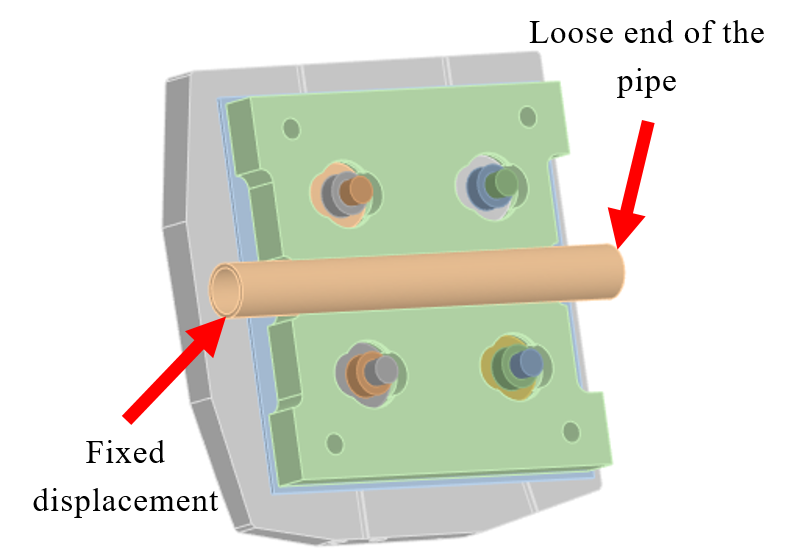
\includegraphics[width=.8\textwidth]{figures/BCStructuralConfig.png}
    \caption{\it Boundary conditions for the reference case (0).}
\end{figure}
\\
\normalsize{\indent For an acurate of the tube and the heat sinks, the whole module ($H-02$) \ref{PlasmaHLonKiPModules} is cut to only feature the two supports on which the reflector tile heat sink is brazed on. The model doesn't feature the graphite/\acrshort{TZM} tiles nor the bolting system to simplifiy the calculations.}
\begin{figure}[!ht]
    \label{fig_5_15} 
    \centering
    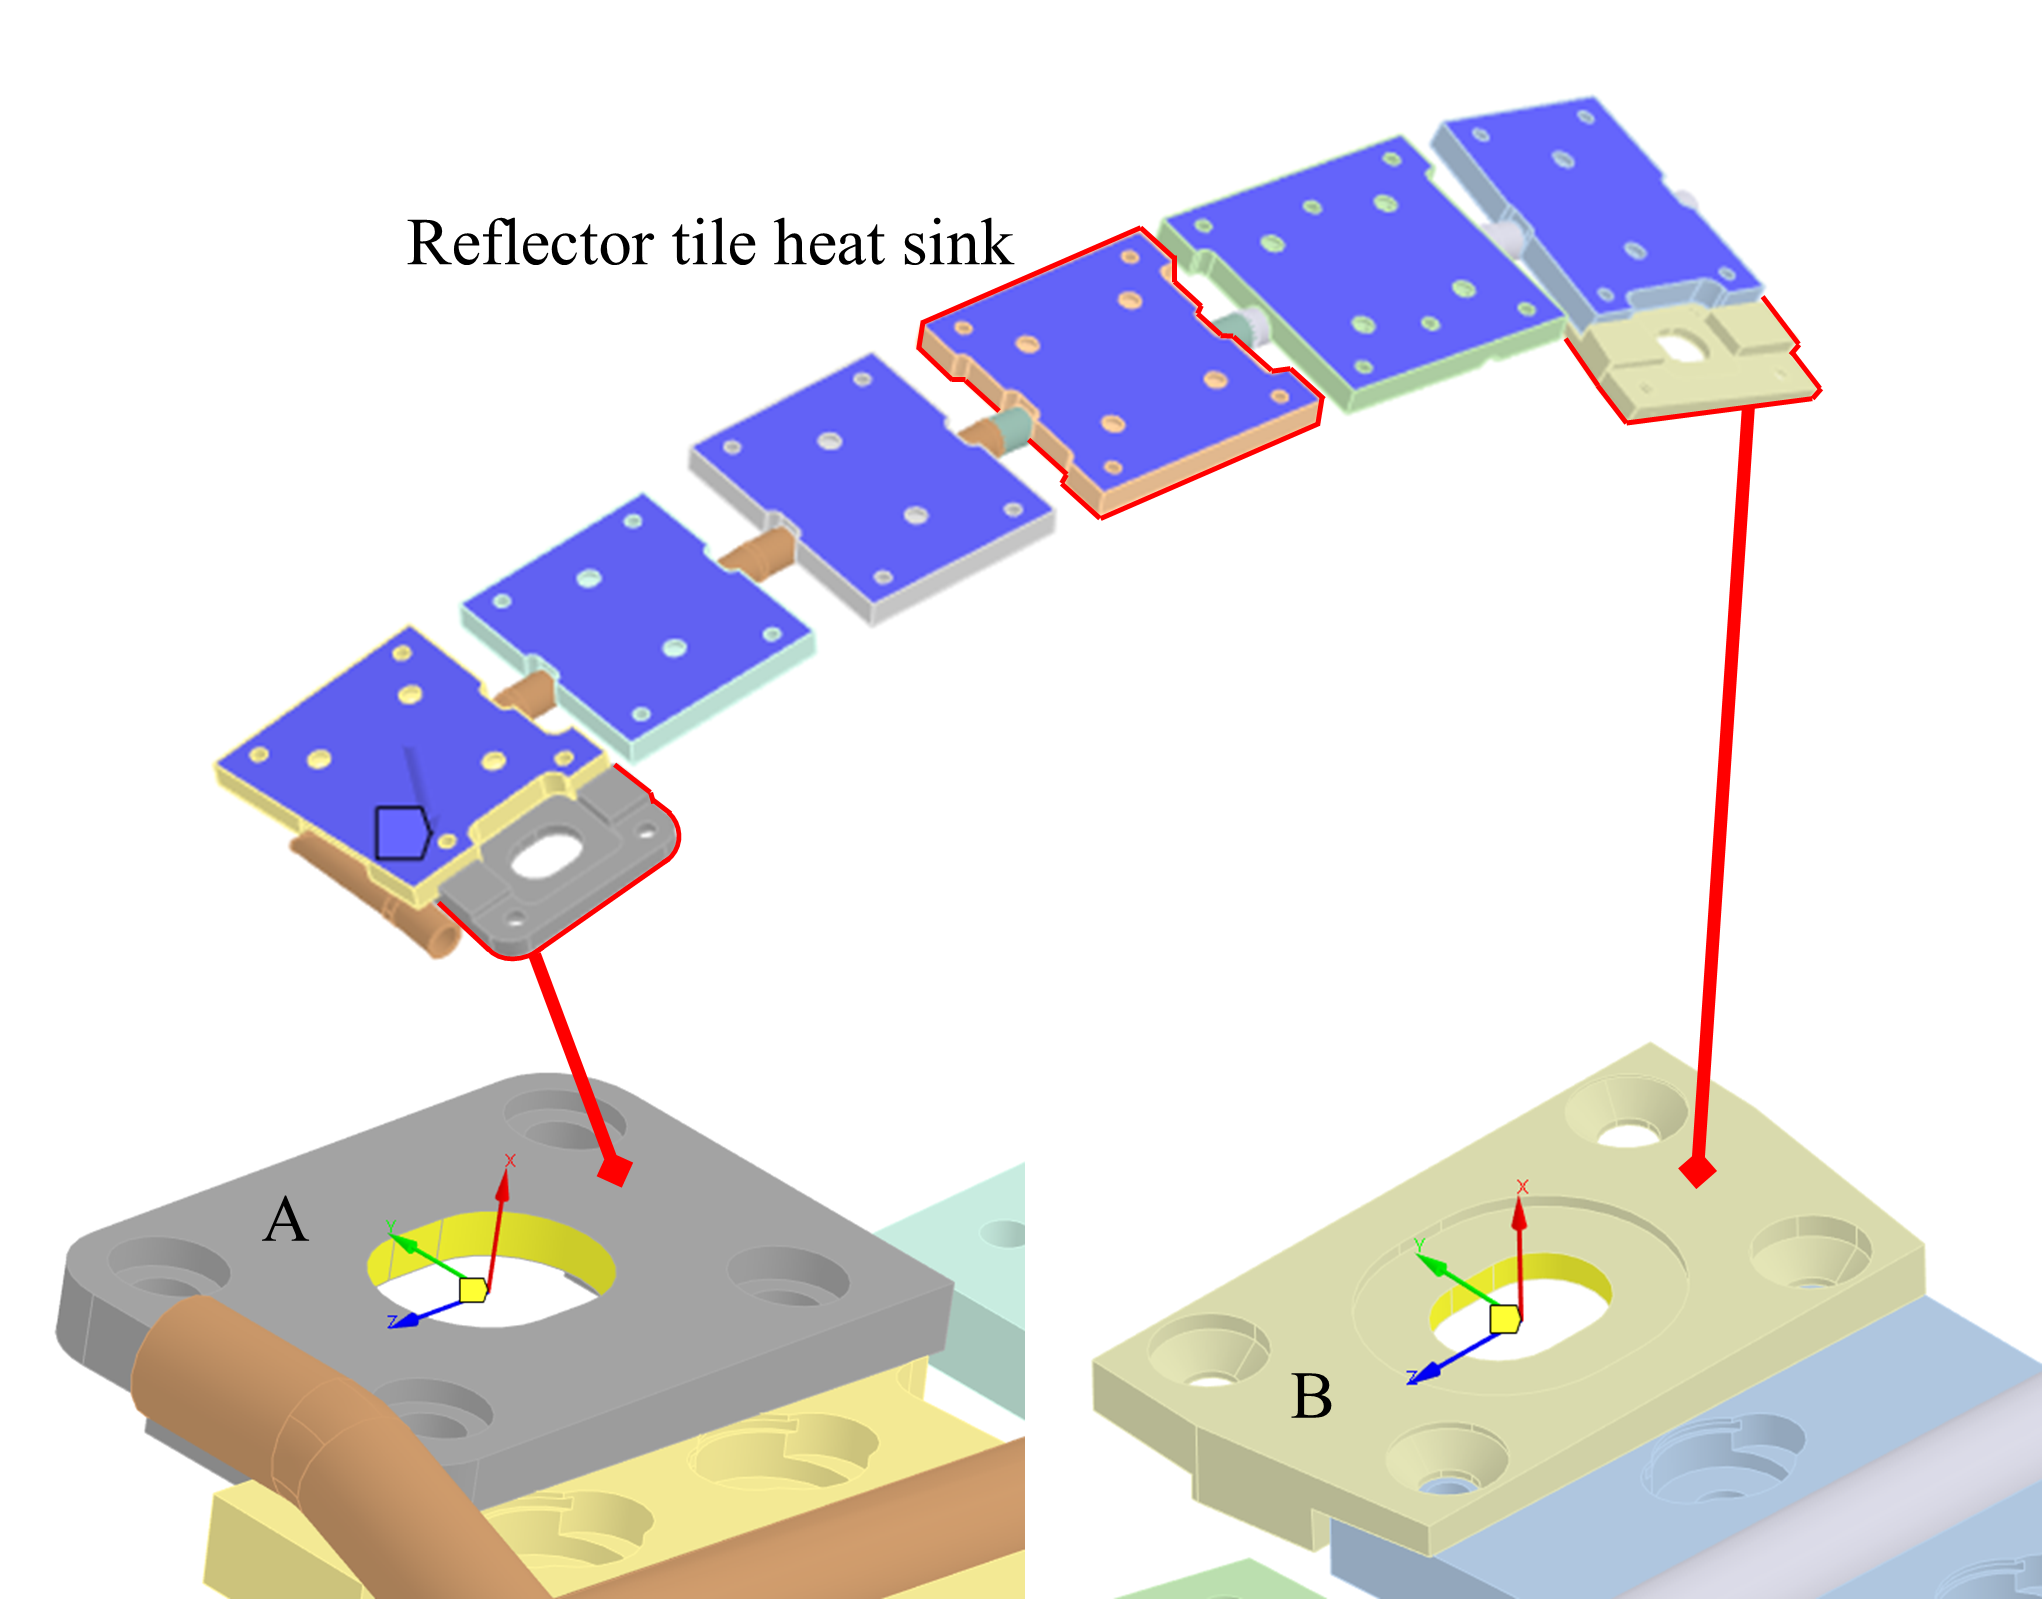
\includegraphics[width=1\textwidth]{figures/one3rdOfModule.png}
    \caption{\it Boun}
\end{figure}
% INSERT TABLE WITH DOF
\subsection{Contact status after calculations with 100 \% contact between TZM-tile and Sigraflex thermal gasket}
